%%%% Paramétrage du TD %%%%
\def\xxactivite{ \ifprof \normalsize{Activation 1 -- Corrigé } \else  \ifcolle Colle \else Activation 1\fi \fi} % \normalsize \vspace{-.4cm}
\def\xxauteur{\textsl{Xavier Pessoles}}


\def\xxnumchapitre{Chapitre 2 \vspace{.2cm}}
\def\xxchapitre{\hspace{.12cm} Hyperstatisme}



\def\xxcompetences{%
\textsl{%
\textbf{Savoirs et compétences :}\\
\begin{itemize}[label=\ding{112},font=\color{ocre}] 
\item \textit{Mod2.C34} : chaînes de solides.
%\item \textit{Mod2.C34} : degré de mobilité du modèle;
%\item \textit{Mod2.C34} : degré d’hyperstatisme du modèle;
%\item \textit{Mod2.C34.SF1} : déterminer les conditions géométriques associées à l’hyperstatisme;
%\item \textit{Mod2.C34} : résoudre le système associé à la fermeture cinématique et en déduire le degré de mobilité et d’hyperstatisme.
\end{itemize}
}}

\def\xxtitreexo{Pompe à chaleur à compresseur Scroll}
\def\xxsourceexo{\hspace{.2cm} XENS -- PSI -- 2018}


\def\xxfigures{
%\includegraphics[width=.7\linewidth]{axe_y_photo}
}%figues de la page de garde


\input{\repRel/Style/pagegarde_TD}
\setcounter{numques}{0}
\setlength{\columnseprule}{.1pt}
\pagestyle{fancy}
\thispagestyle{plain}
\vspace{5.2cm}

\def\columnseprulecolor{\color{ocre}}
\setlength{\columnseprule}{0.4pt} 

%%%%%%%%%%%%%%%%%%%%%%%

\setcounter{exo}{0}
\ifprof
\else


\ifprof
\begin{multicols}{2}
\else
\begin{multicols}{2}
\fi

\subsection*{Présentation}
Le compresseur Scroll utilise deux spirales de géométrie identique emboîtées l’une dans 
l’autre. L’une des spirales est fixe tandis que la seconde est mobile et mise 
en mouvement grâce à un arbre muni d’un excentrique. 

\begin{center}%{H}
%\centering
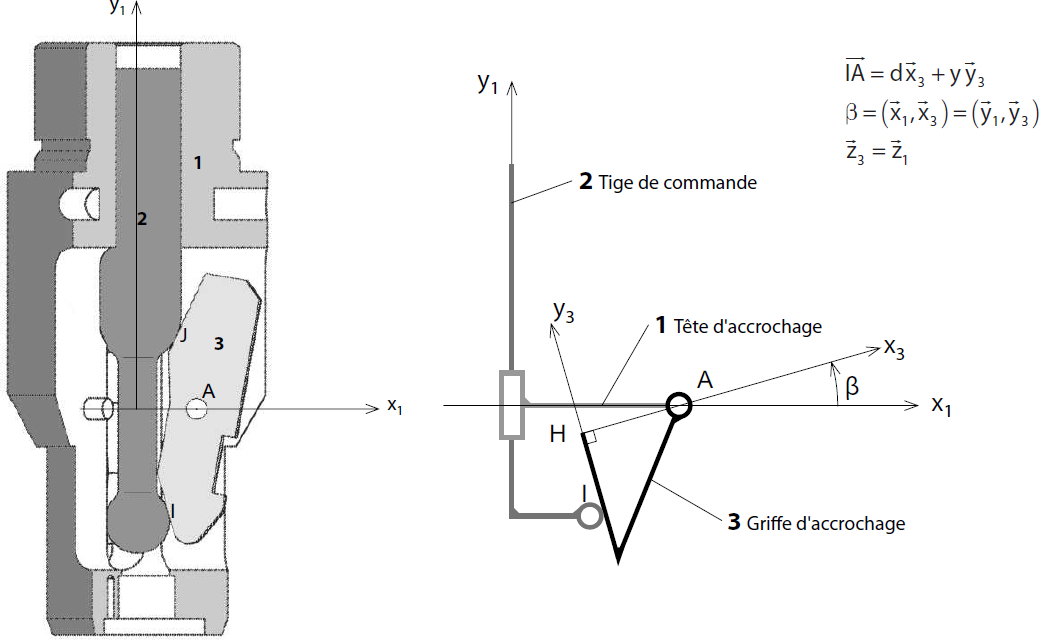
\includegraphics[width=4cm]{fig_01}
\end{center}


\subsubsection*{Etude préliminaire d'un joint de Oldham}


Le joint de Oldham est un accouplement utilisé en général entre 2 axes parallèles mais non-coaxiaux. La figure ci-après en donne les constituants de principe :
\begin{itemize}
\item un arbre d’entrée (noté 1) pouvant tourner autour de l’axe $\axe{O_1}{z_{p1}}$ par rapport à un bâti ;
\item un arbre de sortie (noté 2) pouvant tourner autour de l’axe $\axe{O_2}{z_{p2}}$ par rapport à un bâti ;
\item une pièce intermédiaire appelée en général « noix » ou « croix » (notée 3).
\end{itemize}

\begin{center}%{H}
%\centering
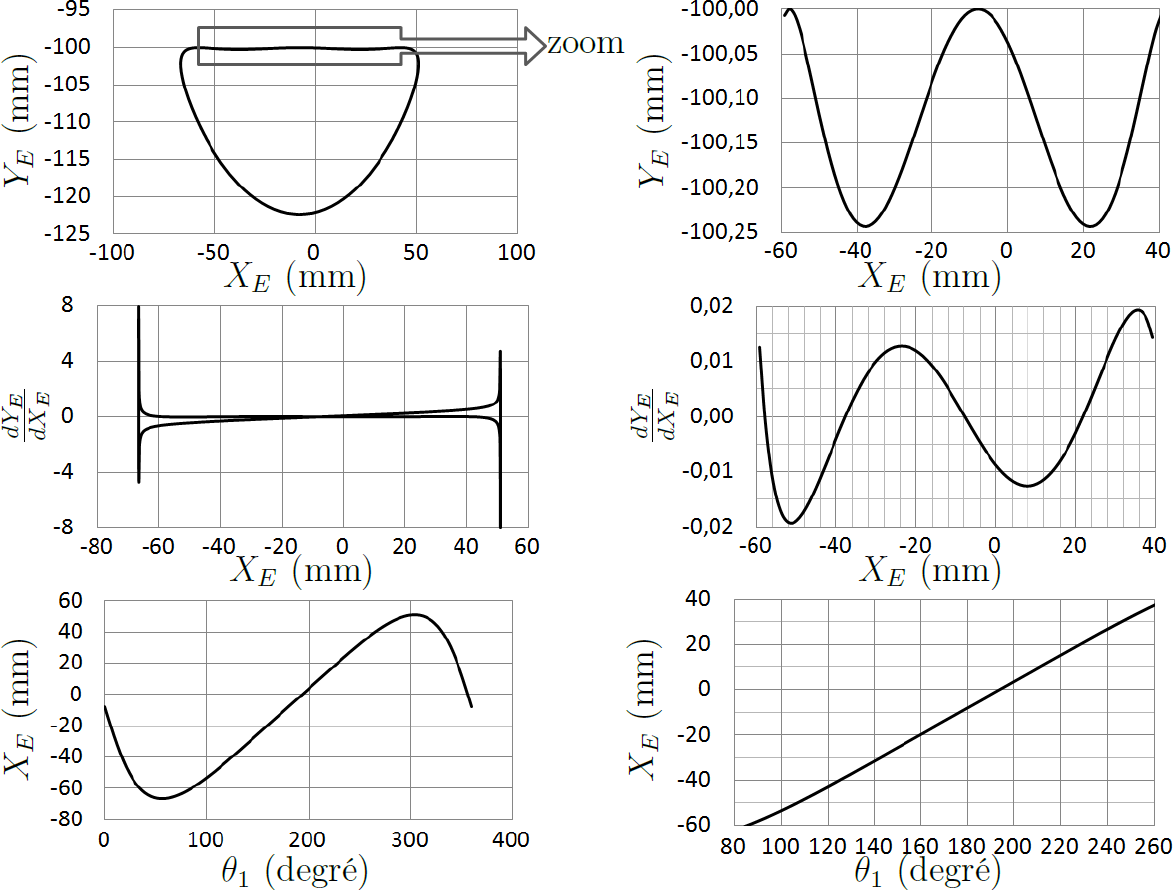
\includegraphics[width=8cm]{fig_03}
\end{center}

La transmission de la rotation de l’arbre 1 à l’arbre 2 est rendue possible par les caractéristiques des liaisons avec la noix 3 : il est nécessaire d’avoir deux glissières orthogonales au niveau de la noix. Ainsi, on retrouve :
\begin{itemize}
\item une glissière de direction $\vect{y_{P1}}$ entre 1 et 3 ;
\item une glissière de direction $\vect{x_{P2}}$ entre 3 et 2.
\end{itemize}

Ces 2 glissières sont par construction constamment orthogonales.

La figure ci-après représente le paramétrage de ce même joint de Oldham avec $\bas{0}\base{x_{P0}}{y_{P0}}{z_{P0}}$ la base fixe liée au bâti 0.

\begin{center}%{H}
%\centering
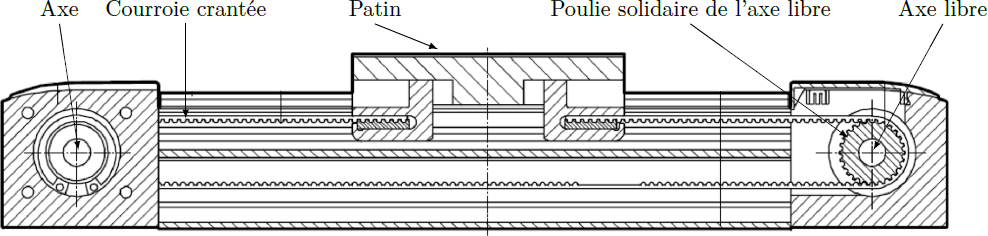
\includegraphics[width=8cm]{fig_04}
\end{center}


Paramétrage :
\begin{itemize}
\item $\vect{O_1 O_2} =  - e\vect{x_{P0}} + h \vect{z_0}$;
\item $\vect{L_1 O_1 }=l_1 \vect{z_P}$;
\item $\vect{O_1 L_2 } =\lambda_2 \vect{y_{P1}}$;
\item $\vect{O_2 L_4 } =l_2 \vect{z_P}$
\item $\vect{L_3 O_2} = \lambda_2  \vect{x_{P2}}$.
\end{itemize}

Les liaisons entre le bâti 0 et les pièces 1 et 2 sont toutes deux des liaisons pivots d’axes respectifs
$\axe{L_1}{z_P}$ et $\axe{L_4}{z_P}$.


\question{Représenter la figure plane de calcul reliant la base $\bas{1}\base{x_{P1}}{y_{P1}}{z_{P0}}$
à la base $\bas{0}$ ainsi que celle reliant la base $\bas{2}\base{x_{P2}}{y_{P2}}{z_{P0}}$ à la base $\bas{0}$.
Exprimer $\vect{y_{P1}}$ et $\vect{x_{P2}}$ dans la base $\bas{0}$ en fonction respectivement de $\theta_1$ et $\theta_2$.}

\question{Étant donnée l’orthogonalité entre $\vect{y_{P1}}$ et $\vect{x_{P2}}$, montrer que $\sin\left(\theta_2 - \theta_1\right)=0$.}

\question{Justifier, à partir du résultat précédent, que l’accouplement en rotation par joint de Oldham soit qualifié de « homocinétique en rotation », c’est-à-dire que le rapport de transmission entre la vitesse de rotation de 1 par rapport à 0, $\omega_1$, et celle de 2 par rapport à 0, $\omega_2$, est constant dans le temps.}

\question{Calculer le degré d’hyperstatisme de ce modèle d’accouplement à partir des grandeurs cinématiques.}

Afin de baisser l’hyperstatisme de l’accouplement, une version alternative est proposée en 
remplaçant les liaisons $L_2$ et $L_3$ par des liaisons pivot-glissant toujours d’axes respectifs
$\axe{O_1}{y_{P1}}$ et $\axe{O_2}{x_{P2}}$.



\question{Vérifier, à partir d’une analyse basée sur les grandeurs statiques, que le degré d’hyperstatisme a bien diminué suite à cette modification.}


\question{Proposer une modification permettant de rendre le système isostatique en conservant sa fonctionnalité.}

\subsection*{Etude cinématique du cpmpresseur Scroll complet}


La vue éclatée présentée sur la figure suivante permet d’identifier les différents composants du compresseur :
\begin{itemize}
\item le bâti fixe composé du carter extérieur, du stator du moteur électrique, de la butée médiane et de la spirale fixe placée en partie haute;
\item l’axe principal composé d’un vilebrequin, du rotor moteur, du contrepoids et de masselottes d’équilibrage;
\item la spirale mobile;
\item la croix.
\end{itemize}

\begin{center}%{H}
%\centering
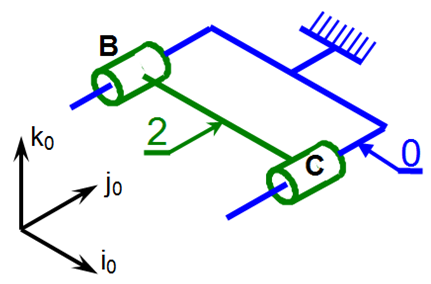
\includegraphics[width=8cm]{fig_02}
\end{center}


Le schéma cinématique proposé reprend les éléments précédents en 
conservant les ensembles cinématiques.
Les contacts entre les spirales fixe et mobile sont négligés dans cette modélisation.

\begin{center}%{H}
%\centering
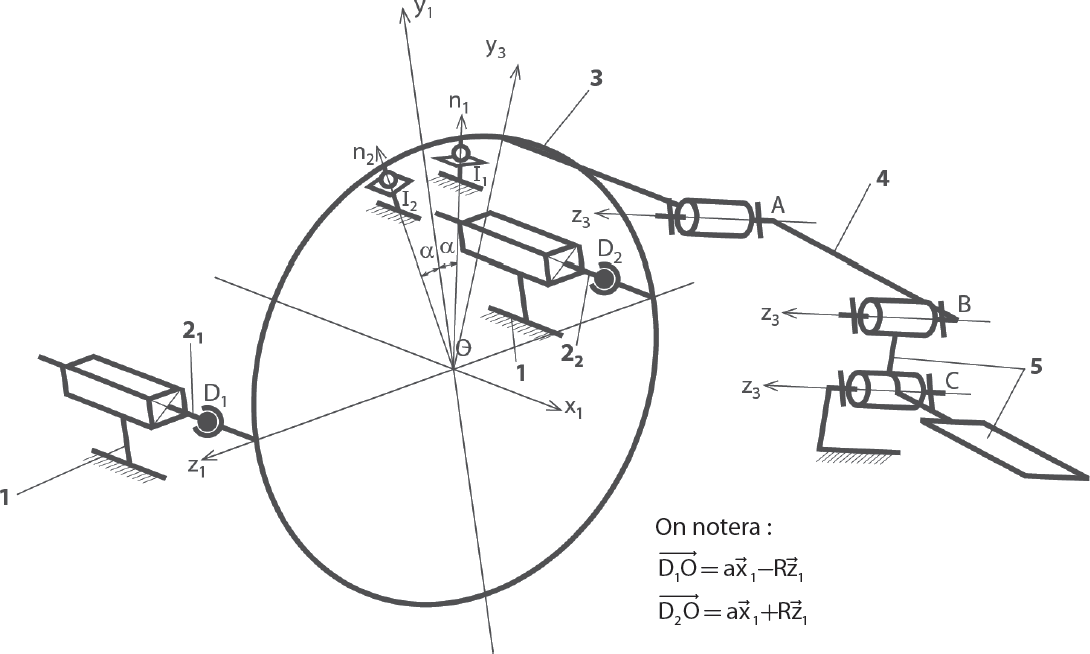
\includegraphics[width=8cm]{fig_05}
\end{center}

\textbf{Paramétrage :}
\begin{itemize}
\item $\rep{0}\repere{O}{x_0}{y_0}{z_0}$ est le repère associé au bâti 0 ;
\item $\rep{1}\repere{O}{x_1}{y_1}{z_1}$ est le repère associé au au vilebrequin 1 :
\begin{itemize}
\item la rotation de $S_1$ par rapport à 0 est repérée par l’angle $\theta = \angl{x_0}{x_1} = \angl{y_0}{y_1}$;
\item la vitesse de rotation est notée $\omega=\thetap = \SI{3600}{tr/min}$.
\end{itemize}
\item $\vect{OA} = a \vect{z_1}$ avec $a=\SI{340}{mm}$;
\item $\vect{AC} =\indice{R}{orb}\vect{x}{1}+d \vect{z_1}$ avec $\indice{R}{orb}=\SI{8}{mm}$ et $d=\SI{80}{mm}$.
\end{itemize}

Liaisons supposées parfaites :
\begin{itemize} 
\item entre le vilebrequin $S_1$ et le bâti 0 :
\begin{itemize}
\item liaison rotule de centre $O$ ;
\item liaison linéaire annulaire de centre $A$ et d’axe $\vect{A}{z_0}$;
\end{itemize}
\item entre le vilebrequin $S_1$ et la spirale mobile $S_2$  :
\begin{itemize}
\item liaison pivot glissant d’axe $\axe{C}{z_0}$;
\end{itemize}
\item entre la spirale mobile $S_2$  et la croix $S_3$  :
\begin{itemize}
\item liaison glissière de direction $\vect{x_0}$;
\end{itemize}
\item entre la croix $S_3$ et le bâti 0 :
\begin{itemize}
\item liaison glissière de direction $\vect{y_0}$.
\end{itemize}
\end{itemize}

Liaison non parfaite :
\begin{itemize}
\item entre la spirale mobile  $S_2$ et le bâti 0 :
\begin{itemize}
\item liaison appui-plan avec frottement de normale $\vect{z_0}$.
\end{itemize}
\end{itemize}

\question{Tracer le graphe des liaisons du système tel que modélisé sur la Figure précédente en faisant apparaître chaque liaison avec ses caractéristiques.}

\question{Démontrer par le calcul que l’association des liaisons en $O$ et en $A$ entre le vilebrequin et le carter forme une liaison pivot d’axe $\axe{O}{z_1}$.}


\question{Indiquer la valeur de l’indice de mobilité du système dans cette modélisation à  partirà partir de l’analyse du schéma cinématique. Proposer une démarche qui, sans utiliser le degré d’hyperstatisme du système, permettrait de retrouver analytiquement cette valeur.}

Il est intéressant de remarquer que la croix $S_3$ réalise un accouplement de type joint de Oldham entre la spirale mobile $S_2$ et le bâti 0.

\question{Justifier alors que la vitesse de rotation de $S_2$ par rapport à 0 est nulle.}

\question{Exprimer, dans la base $\bas{1}$, la vitesse instantanée du point $C$ appartenant à $S_2$ dans son mouvement par rapport à 0. Faire l’application numérique.}

\question{Déduire des questions précédentes le type de mouvement de la spirale mobile $S_2$ dans son déplacement par rapport à 0 ainsi que ses qualificatifs et caractéristiques.}


\ifprof
\end{multicols}
\else
\end{multicols}
\fi

